\subsection{Sequence Diagram}

\begin{figure}[H]
    \centering
    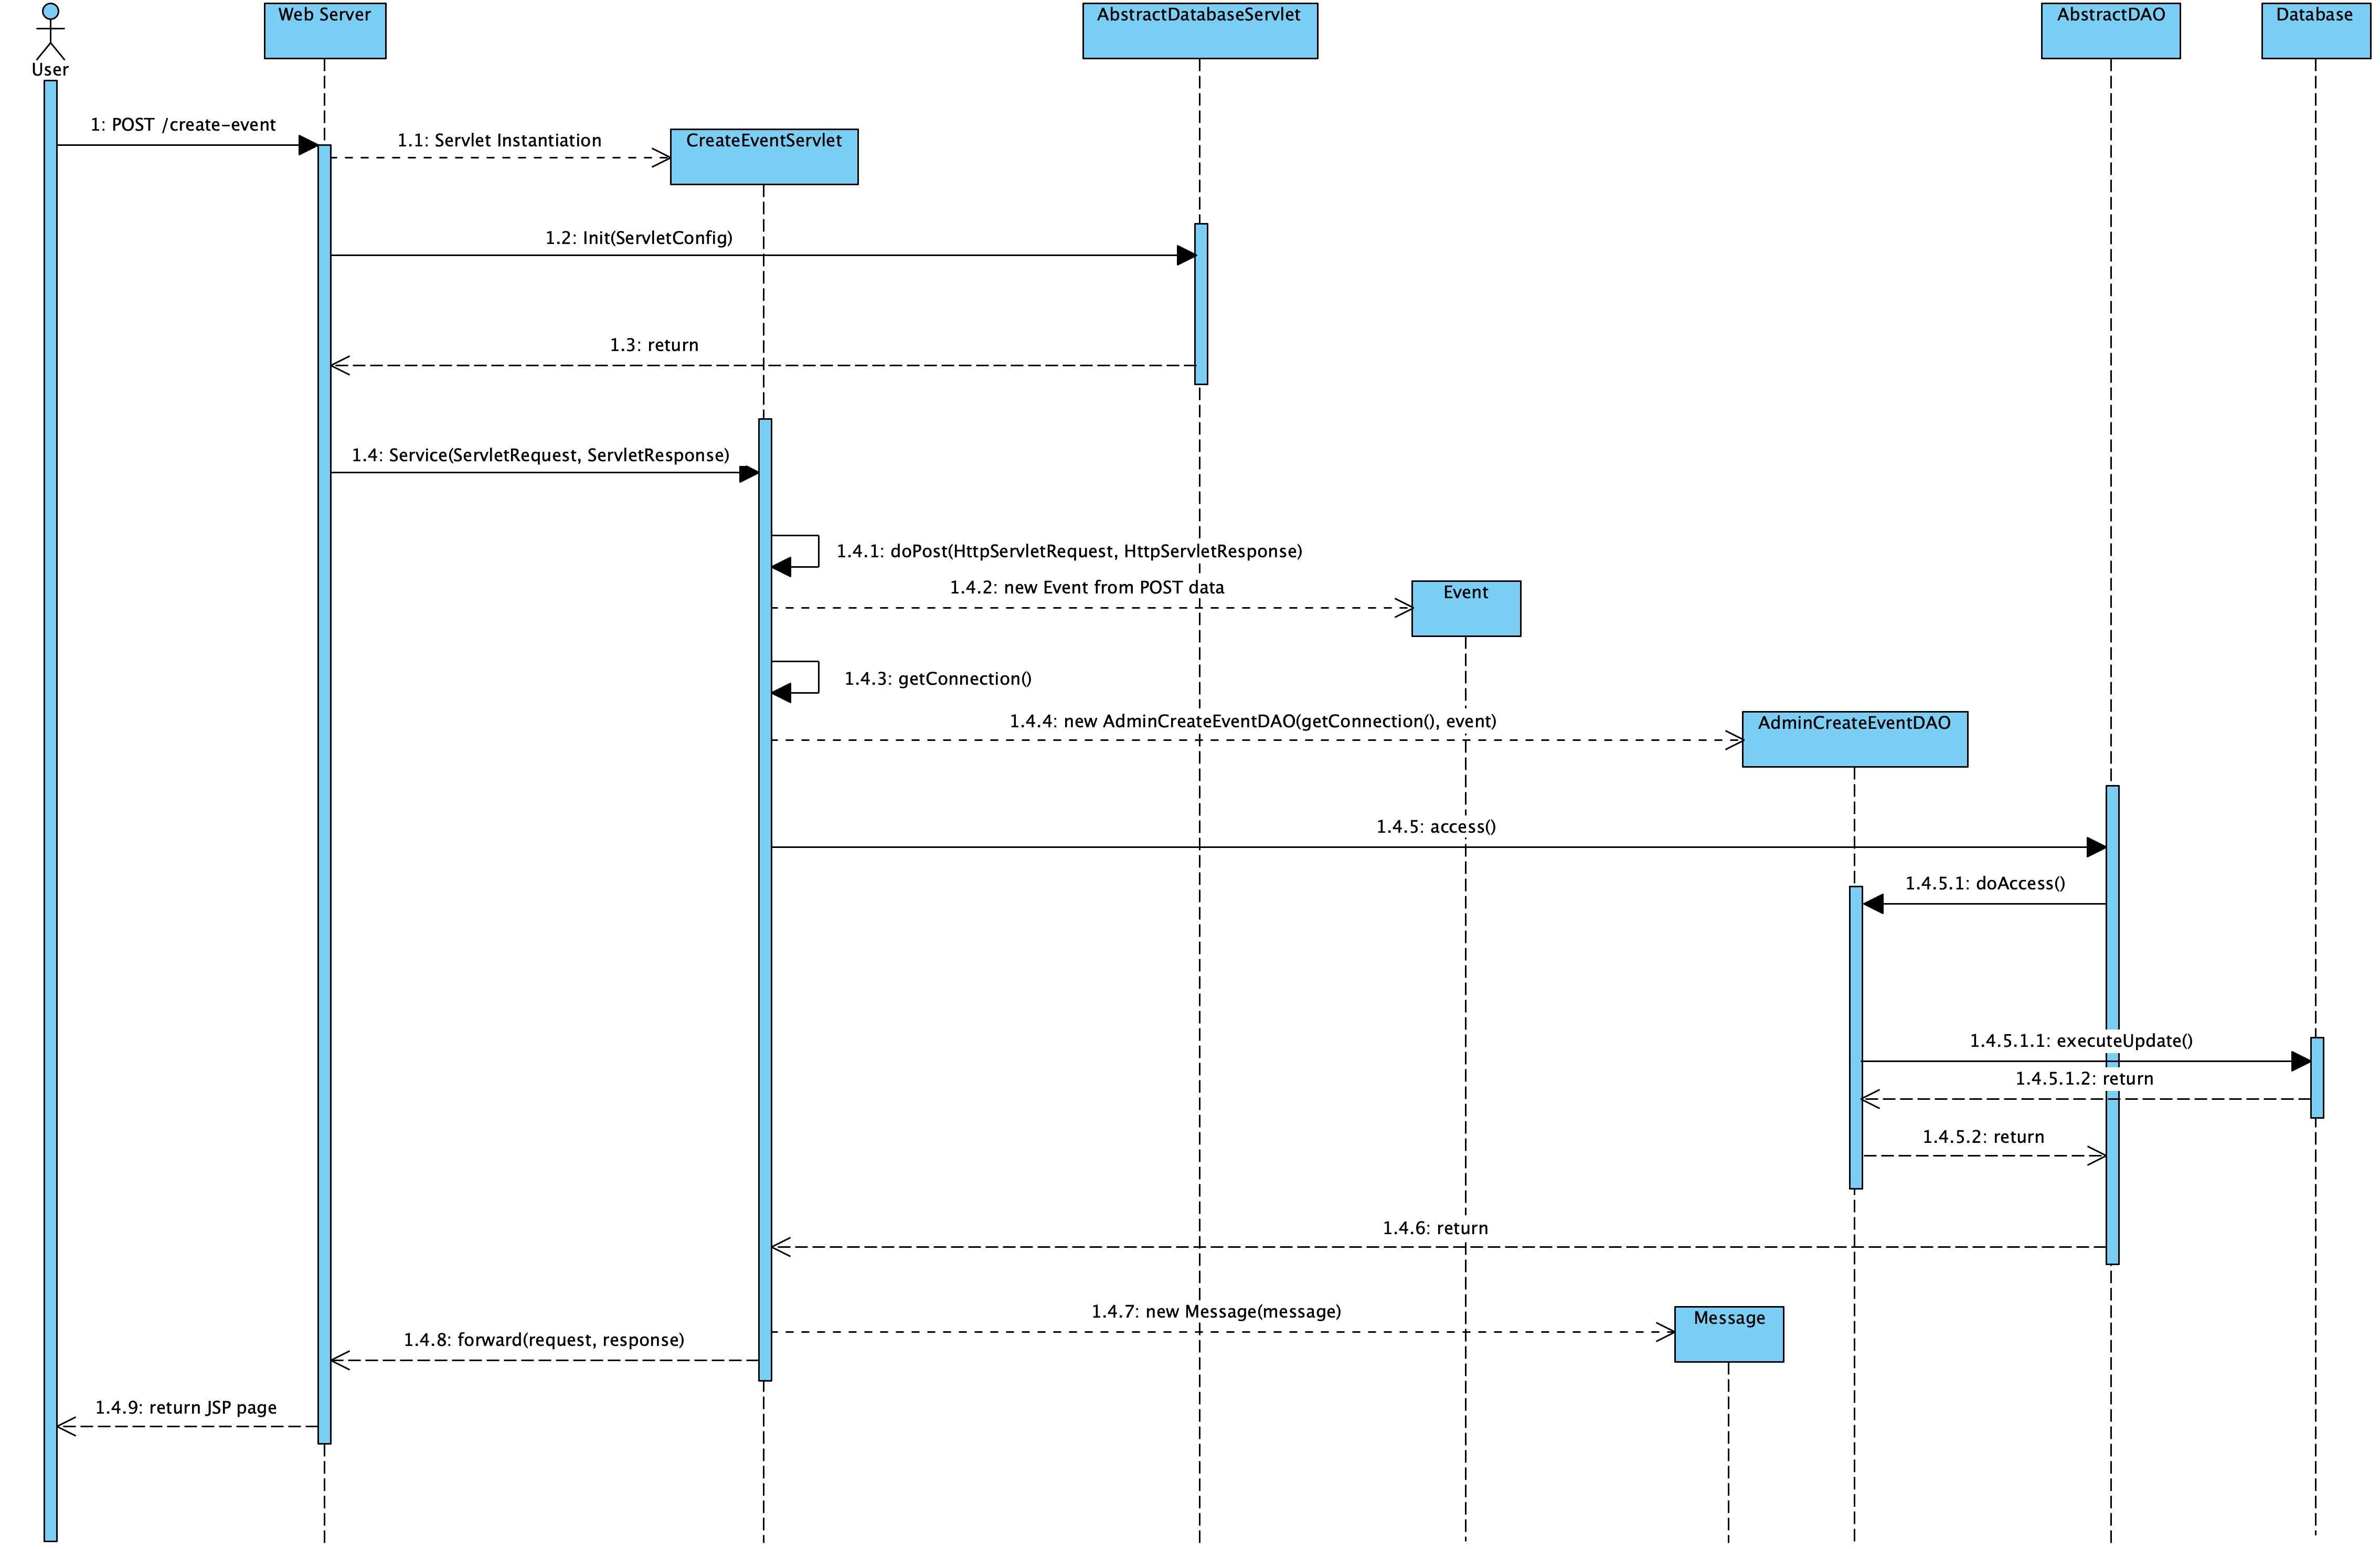
\includegraphics[width=1\textwidth]{images/CreateEventSequence.png}
    \caption{Create Event Sequence Diagarm}
    \label{fig:create event sequence diagram}
\end{figure}

%describe here the sequence diagram
Here reported the sequence diagram for the event creation operation.
To create a new event, an Admin user (at least tier 3), fills the creation form in the Create Event page.
By clicking on Continue button, a POST request is issued to the web server, specifying the URI: /create-event. \\
The data passed to the web server are name, description, price, visibility, place (city, street and number),
maximum number of international participants, maximum number of volunteer participants, start date, end date,
start subscription date, end subscription date, withdrawal end date, size of waiting list, attributes,
thumbnail image and poster image. \\
The web server instantiates the CreateEventServlet which calls its doPost method, passing the HttpServletRequest
and HttpServletResponse. This method handles some POST data packing city, street and number in a unique location JSON
Object and storing the two images (thumbnail and poster) in the “ESSENTLS\_Cloud” folder.
A new Event object is created, containing the other POST data, the generated location JSON object and the paths that
represent the images. The control is passed to the AdminCreateEventDAO which receives as arguments the connection
(defined in the AbstractDatabaseServlet extended by the CreateEventServlet) and the instantiated Event.
The AdminCreateEventDAO (that extends the AbstractDAO ) contacts the Database Server with the access() method that
calls the doAccess() override method in the AdminCreateEventDAO, which executes the SQL statement for event creation.
The operation ends returning a message that informs the user that the event is successfully created.